\section{Spotting Qualitative Differences between Supervised and Unsupervised NMT with \maf1}
\label{sec:unmt}

% \begin{tabular}{l rr | rr | rr| rr | rr | rr }
% \multicolumn{1}{}{} 
%      & \multicolumn{2}{c|}{\bleu}
%                   & \multicolumn{2}{c|}{\maf1} 
%                                  & \multicolumn{2}{c|}{\mif1} 
%                                               &\multicolumn{2}{c|}{\chrf1} 
%                                                             &\multicolumn{2}{c|}{\blrtmn} 
%                                                                                 &\multicolumn{2}{c}{\blrtmd} \\
%      & SN   & UN   & SN   & UN   & SN   & UN   & SN   & UN   & SN     & UN      & SN     & UN \\ \hline\hline
% DEEN & 32.7 & 33.9 & 38.5 & 33.6 & 58.7 & 57.9 & 59.9 & 58.0 & 0.211 & -0.026 & 0.285 & 0.067 \\
% ENDE & 24.0 & 24.0 & 24.0 & 23.5 & 47.7 & 48.1 & 53.3 & 52.0 &-0.134 & -0.204 &-0.112 & -0.197 \\
% FREN & 31.1 & 31.2 & 41.6 & 33.6 & 60.5 & 58.3 & 59.1 & 57.3 & 0.182 &  0.066 & 0.243 & 0.154 \\
% ENFR & 25.6 & 27.1 & 31.9 & 27.4 & 53.0 & 52.3 & 56.0 & 57.7 & 0.104 &  0.042 & 0.096 & 0.063 \\
% ROEN & 30.8 & 29.6 & 40.3 & 33.0 & 59.8 & 56.5 & 58.0 & 54.7 & 0.004 & -0.058 & 0.045 &-0.004 \\
% ENRO & 31.2 & 31.0 & 34.6 & 31.0 & 55.4 & 53.4 & 59.3 & 56.7 & 0.030 & -0.046 & 0.027 &-0.038 \\ 
% \end{tabular}%
\begin{table*}[ht!]
\centering
%\fontsize{8.5}{8.8}
%\selectfont
\footnotesize

\begin{tabular}{l @{\hspace{3mm}} r @{\hspace{1.5mm}} r @{\hspace{1.5mm}}r |  r@{\hspace{1.5mm}}r@{\hspace{1.5mm}}r |
  r@{\hspace{1.5mm}}r@{\hspace{1.5mm}}r | r@{\hspace{1.5mm}} r@{\hspace{1.5mm}} r | r@{\hspace{1.5mm}} r@{\hspace{1.5mm}} r | r @{\hspace{1.5mm}} r@{\hspace{1.5mm}} r}
& \multicolumn{3}{c|}{\bleu} & \multicolumn{3}{c|}{ \maf1 } & \multicolumn{3}{c|}{ \mif1 } & \multicolumn{3}{c|}{ \chrf1 } & \multicolumn{3}{c|}{ \blrtmn } & \multicolumn{3}{c}{ \blrtmd } \\ 
& SN & UN & $\Delta$ & SN & UN & $\Delta$ & SN & UN & $\Delta$ & SN & UN & $\Delta$ & SN & UN & $\Delta$ & SN & UN & $\Delta$ \\ \hline \hline
DE-EN & 32.7 & 33.9 & -1.2 & 38.5 & 33.6 & 4.9 & 58.7 & 57.9 &  0.8 & 59.9 & 58.0 &  1.9 & .211 & -.026 & .24 & .285 & .067 & .22 \\
EN-DE & 24.0 & 24.0 &  0.0 & 24.0 & 23.5 & 0.5 & 47.7 & 48.1 & -0.4 & 53.3 & 52.0 &  1.3 &-.134 & -.204 & .07 &-.112 &-.197 & .09 \\
FR-EN & 31.1 & 31.2 & -0.1 & 41.6 & 33.6 & 8.0 & 60.5 & 58.3 &  2.2 & 59.1 & 57.3 &  1.8 & .182 &  .066 & .17 & .243 & .154 & .09 \\
EN-FR & 25.6 & 27.1 & -1.5 & 31.9 & 27.3 & 4.6 & 53.0 & 52.3 &  0.7 & 56.0 & 57.7 & -1.7 & .104 &  .042 & .06 & .096 & .063 & .03 \\
RO-EN & 30.8 & 29.6 &  1.2 & 40.3 & 33.0 & 7.3 & 59.8 & 56.5 &  3.3 & 58.0 & 54.7 &  3.3 & .004 & -.058 & .06 & .045 & -.004 & .04 \\
EN-RO & 31.2 & 31.0 &  0.2 & 34.6 & 31.0 & 3.6 & 55.4 & 53.4 &  2.0 & 59.3 & 56.7 &  2.6 & .030 & -.046 & .08 & .027 & -.038 & .07 \\
\end{tabular} 

\caption{For each language direction, UNMT (UN) models have similar \bleu\ to SNMT (SN) models, and \chrf1 and \mif1 have small differences. 
However, \maf1 scores differ significantly, consistently in favor of SNMT. 
Both corpus-level interpretations of BLEURT support the trend reflected by \maf1, but the value differences are difficult to interpret.
}
\label{tab:unmt_vs_snmt}
\end{table*}

% \begin{figure*}[ht!]
%     \centering
%     \begin{subfigure}[b]{0.48\linewidth}
%     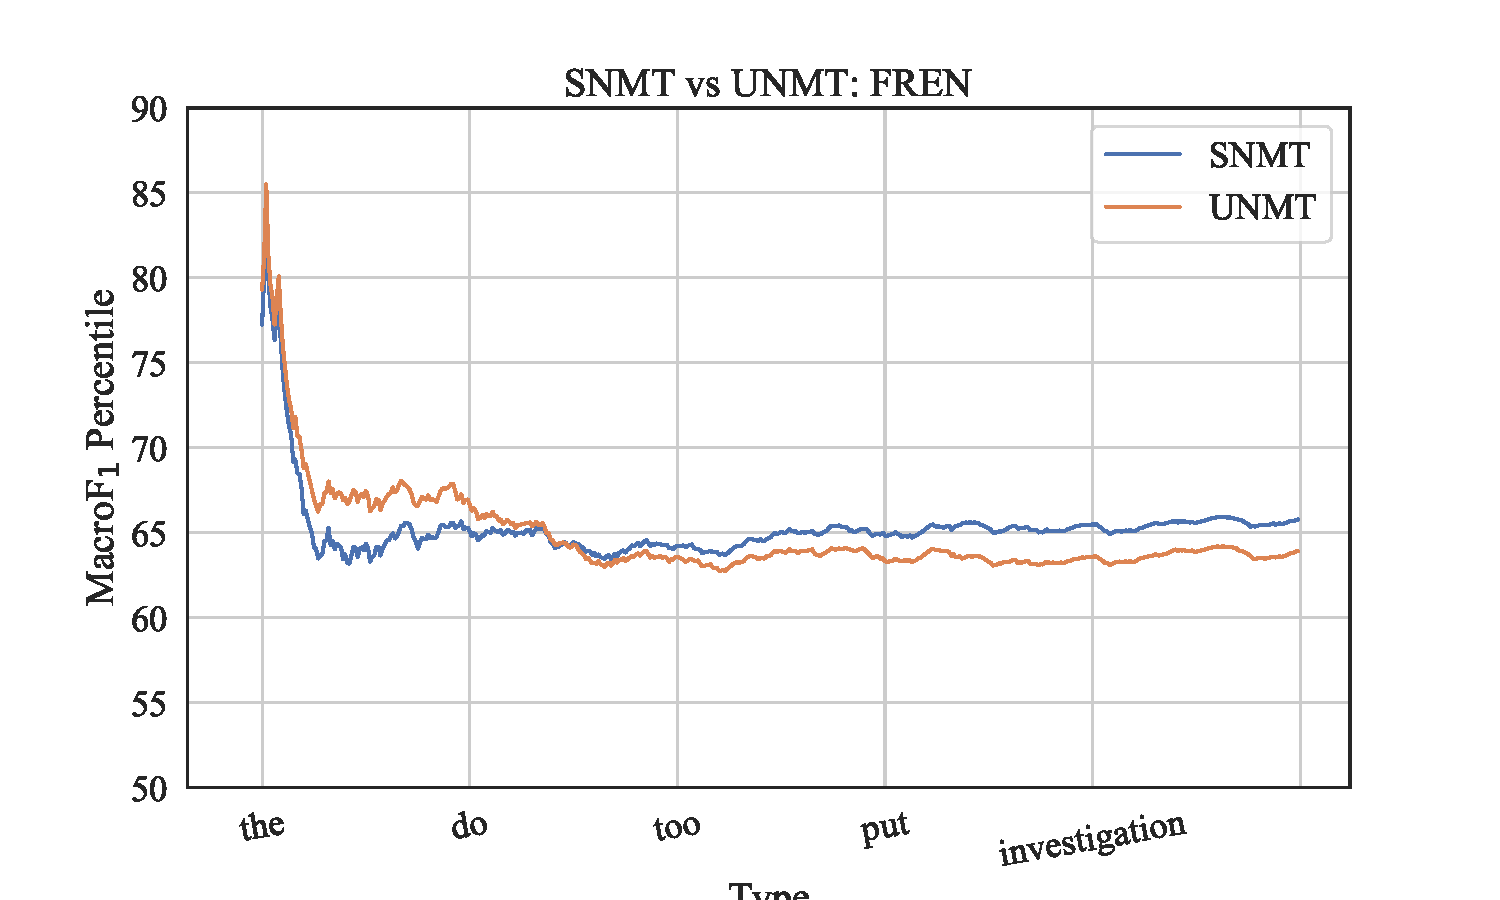
\includegraphics[width=\linewidth,trim={13mm 5mm 25mm 10mm},clip]{img/s_unmt-fren-maf1.pdf}
%     \label{fig:s-vs-u-fren}
%     \end{subfigure}
%     \hfill 
%     \begin{subfigure}[b]{0.48\linewidth}
%     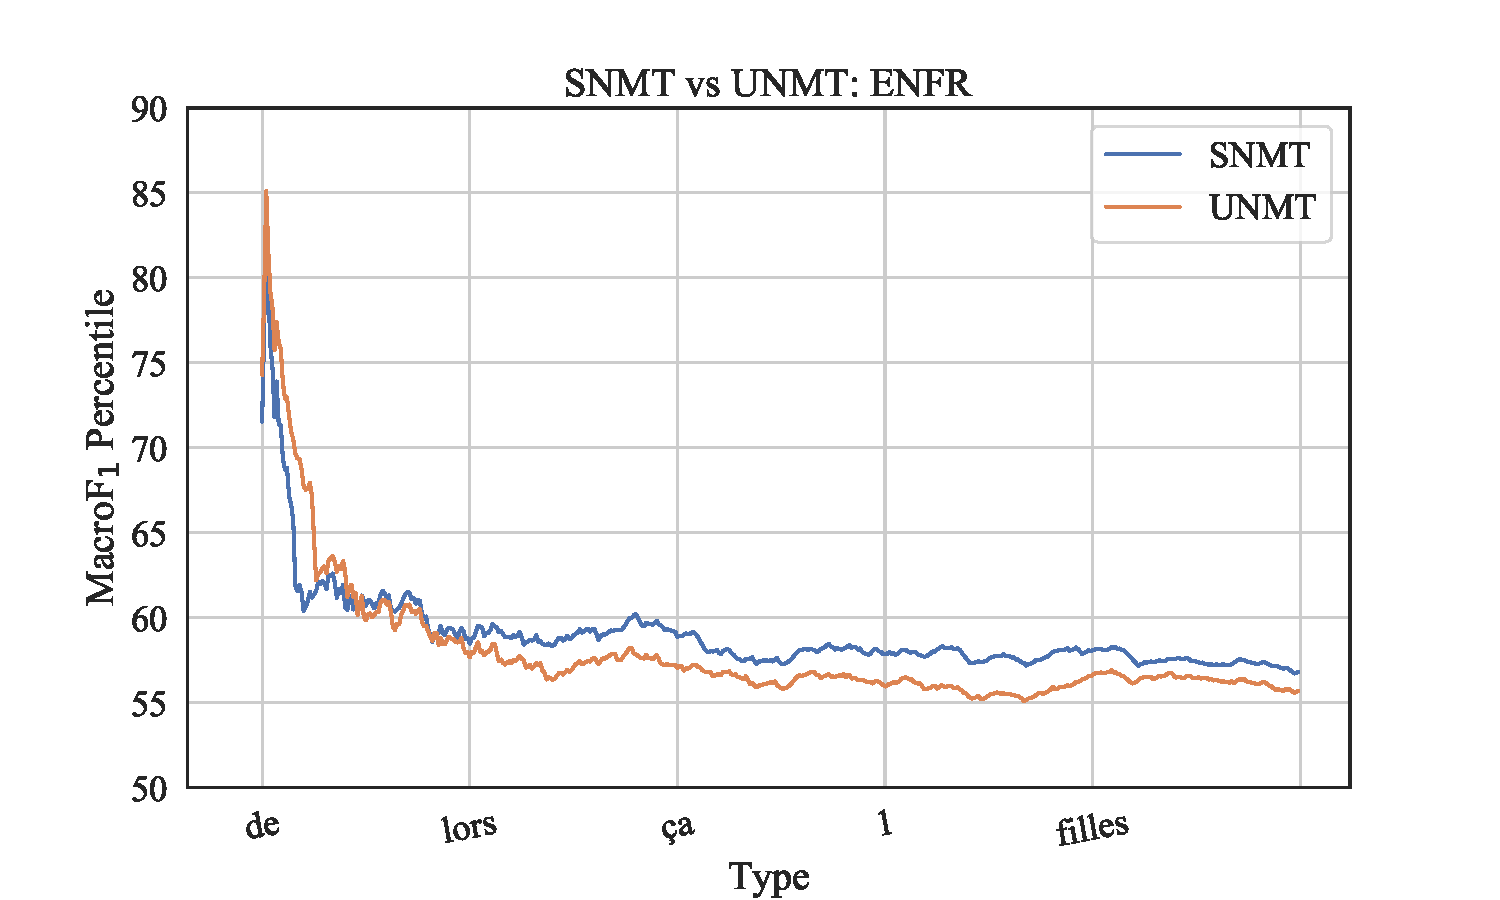
\includegraphics[width=\linewidth,trim={13mm 7mm 25mm 10mm},clip]{img/s_unmt-enfr-maf1.pdf}
%     \label{fig:s-vs-u-roen} 
%     \end{subfigure}

% \caption{\small Visualization of \maf1 between SNMT and UNMT. 
% Only the FREN and ENFR test sets for the most frequent 500 types are shown here, but the trend is similar on the other settings (see Figure~\ref{fig:snmt_vs_unmt-rest} in appendix).
% UNMT generally outperforms SNMT on the frequent types that contribute to fluency and hence score comparable \bleu\ scores, however, SNMT is generally better than UNMT on rare types hence SNMT scores higher \maf1. \tg{Explain that lines are viz of cumulative .}
% }
% \label{fig:snmt_vs_unmt}
% \end{figure*}

Unsupervised neural machine translation (UNMT) systems trained on massive monolingual data without parallel corpora have made significant progress recently \cite{Artetxe-2018-unmt-iclr,Lample-2018-unmt-iclr,lample-etal-2018-phrase-unmt,yang-etal-2018-unmt,conneau-NIPS2019-xlm,Song-2019-MASS,liu2020mbart}. 
In some cases, UNMT yields a \bleu\ score that is comparable with strong\footnote{though not, generally, the strongest} supervised neural machine translation (SNMT) systems. In this section we leverage \maf1 to investigate differences in the translations from UNMT and SNMT systems that have similar \bleu.

%\subsection{Experiment Settings}
We compare UNMT and SNMT for English $\leftrightarrow$ German (EN-DE, DE-EN), English $\leftrightarrow$ French (EN-FR, FR-EN), and English $\leftrightarrow$ Romanian (EN-RO, RO-EN).
All our UNMT models are based on XLM \citep{conneau-NIPS2019-xlm}, pretrained by \citet{XLM-UNMT-Models20}. 
We choose SNMT models with similar \bleu\ on common test sets by either selecting from systems submitted to previous WMT News Translation shared tasks~\cite{bojar-EtAl:2014:W14-33,bojar-EtAl:2016:WMT1} or by building such systems.\footnote{We were unable to find EN-DE and DE-EN systems with comparable \bleu\ in WMT submissions so we built standard Transformer-base~\cite{vaswani2017attention} models for these using appropriate training data to reach the desired \bleu\ performance. We report EN-RO results with diacritic removed to match the output of UNMT.} Specific SNMT models chosen are in the Appendix (Table~\ref{tab:unmt_vs_snmt2}).

 Table~\ref{tab:unmt_vs_snmt} shows performance for these language pairs using a variety of metrics. Despite comparable \bleu\ and only minor differences in \mif1 and \chrf1, SNMT models have consistently higher \maf1 and BLEURT than the UNMT models for all six translation directions. 
 
% We thus investigate \textit{why} there is such a divergence of relative opinion as measured by these autoeval methods.
% Note that \bleu\ and \chrf1 do not facilitate an type-wise comparison of MT models.
% Even though \blrtmn\ and \blrtmd\ show discrepancy between SNMT and UNMT, we are unable to interpret the difference and reason about it, which is concerning.
% However, \maf1 also provides performance per type, which are readily interpretable, on which macro-average is computed.

% Figure~\ref{fig:snmt_vs_unmt}, which is a visualization of \maf1 on most frequent 500 types, shows that UNMT outperforms SNMT on the frequent types such as stopwords which are weighed relatively highly in \bleu\ and other micro-averaged methods; however, SNMT is generally better than UNMT on the rest; hence, SNMT scores higher \maf1 than UNMT.
% Figure~\ref{fig:snmt_vs_unmt} is a simple explanation for the discrepancy between \maf1 and other micro-averaged methods in Table~\ref{tab:unmt_vs_snmt}.
% The take away from this section is that the easier interpretability aspect of \maf1 helps in uncovering the differences and flaws of MT models.
% For instance, it enabled us to find that the current UNMT systems produce fluent translations where as SNMT systems produce more adequate translations.


\subsection{Pairwise Maximum Difference Discriminator}

We consider cases where a metric has a strong opinion of one translation system over another, and analyze whether the opinion is well justified. In order to obtain this analysis we employ a pairwise segment-level discriminator from within a corpus-level metric, which we call \textit{favoritism}.

%describe a UNMT and SNMT differ in \maf1 to see how \maf1 successfully discriminates MT outputs of different quality. To select extreme cases using a corpus-level metric, we use a pairwise maximum difference discriminator which we define below.

% \begin{table}[t]
%     \centering
%     \footnotesize
%     \begin{tabular}{ll}
% SNMT & UNMT \\ \hline\hline
% synonym&	\textit{untranslation}, \textit{wrong\_noun}\\
% synonym&	\textit{untranslation}\\
% synonym&	\textit{untranslation}, \textit{wrong\_noun}\\
% synonym, word\_order&	\textit{depend}, \textit{trunc}, \textit{word\_order}\\
% synonym, inflection&	\textit{untranslation}, \textit{wrong\_noun}\\
% inflection, word\_order&	\textit{number}\\
% \textit{time}, word\_order&	 \textit{time}, \textit{weird\_char}, synonym\\
% synonym&	\textit{untranslation}, \textit{wrong\_noun}\\
% punctuation, synonym&	\textit{trunc}\\
% synophrase, word\_order&	word\_order, \textit{untranslation}\\
%     \end{tabular}
%     \caption{Problems for top 10 $\delta_{\maf1} (x; S, U)$ sentences such that \maf1 favors SNMT over UNMT for DEEN. The labels in italics are real problems, while the others are issues that hurt \maf1 but are not real translation errors. UNMT has a lot of untranslations.}
%     \label{tab:snmt_better_mf1}
% \end{table}


% \begin{table}[t]
%     \centering
%     % \scalebox{0.8}{
%     \footnotesize
%     \begin{tabular}{ll}
    
% SNMT & UNMT \\ \hline\hline
% \textit{unrelated\_other\_lang}&\\
% \textit{untranslation}&\\
% \textit{omit\_verb}, \textit{untranslation}&	\textit{wrong\_adj}, \textit{wrong\_verb}\\
% \textit{wrong\_name}&	\textit{word\_order}\\
% synophrase, \textit{punctuation}&	\textit{punctuation}, \textit{untranslation}\\
% \textit{trunc}, \textit{wrong\_meaning}&	\textit{untranslation}\\
% synonym, \textit{wrong\_name}&	\textit{omit\_verb}, \textit{wrong\_adj}\\
% \textit{unk}, \textit{untranslation}&	\\
% punctuation, \textit{preposition}&\\
% \textit{trunc}, \textit{extra}&	\textit{extra}\\ 
%     \end{tabular}
%     % }
%     \caption{Problems for bottom 10 $\delta_{\maf1} (x; S, U)$ sentences such that \maf1 favors UNMT over SNMT for DEEN. SNMT has a mixture of wrong words, synonym, and word order problems.}
%     \label{tab:unmt_better_mf1}
% \end{table}



% \begin{table}[t]
%     \centering
%     \footnotesize
%     \begin{tabular}{l @{\hspace{1mm}} r @{\hspace{1mm}} |p{2.5cm} @{\hspace{1mm}} | p{2.5cm} }
% Fav. & $|\delta|$ & SNMT errors  & UNMT errors                            \\ \hline \hline
% S & .71     & syn                    & \textit{untrans}, \textit{wrong}                 \\
% S & .64     & syn                    & \textit{untrans}                              \\
% U & .55     & \textit{unrelated\_other\_lang}       &                                            \\
% S & .52     & syn                     & \textit{untrans}, \textit{wrong}                 \\
% U & .45     & untranslation                &                                            \\
% S & .44     & syn, word\_order         & \textit{subject}, \textit{trunc}, \textit{word\_order}           \\
% S & .44     & syn, tense               & \textit{untrans}, \textit{wrong}                 \\
% S & .43     & inflection, word\_order  & \textit{number}                                     \\
% U & .41     & \textit{omit\_verb}, \textit{untrans}    & \textit{wrong}, \textit{wrong}                    \\
% S & .41     & \textit{wrong}, word\_order & \textit{wrong}, time\_system, \textit{weird\_char}
% \end{tabular}
%     \caption{Problems for top 10 $|\delta_{\maf1} (i; h_S, h_U)|$ for DEEN.}
%     \label{tab:snmt_better_mf1}
% \end{table}

% \begin{table}[ht!]
%     \centering
%     \footnotesize
%     \begin{tabular}{r @{\hspace{2mm}} l @{\hspace{2mm}} p{0.68\linewidth} }
%  $\delta_{\maf1}$ & Fav & Analysis \\ \hline \hline
%  0.71   & S  & S has synonym; U has \textit{untranslation}, and \textit{wrong noun}  \\
%  0.64   & S  & S has synonym; U has \textit{untranslation} \\
%  -0.55  & U  & S has \textit{wrong translation};  U has no issues     \\
%  0.52   & S  & S has synonym; U has \textit{untranslation}, and \textit{wrong noun} \\
%  -0.45  & U  & S has \textit{untranslation}; U has no issues \\
%  0.44   & S  & S has synonym, wrong word order; U has \textit{wrong subject}, \textit{truncation}, and wrong word order \\
%  0.44   & S  & S has synonym and tense issues; U has \textit{untranslation} \\
%   0.43  & S  & S has inflection, and wrong word order ; U has \textit{wrong number} \\
%  -0.41  & U  & S has \textit{omitted verb}, and \textit{untranslation} ; U has \textit{wrong adjective} and \textit{verb} \\
% 0.41    & S & S has \textit{wrong time} and wrong word order; U has \textit{wrong time}, and \textit{wrong nouns} 
% \end{tabular}
% %\caption{Problems in the top 10 segments identified by $|\delta_{\maf1} (i; h_S, h_U)|$ for DEEN. S and U are short for SNMT and UNMT. Fav is the favored system by \maf1. Examples shown in Table~\ref{tab:maf1-top-10}.}
%     \label{tab:snmt_better_mf1}
% %\end{table}

% \vspace{10px}
% %\quad
% %\begin{table}[ht]
% %\centering
% %    \footnotesize
%     \begin{tabular}{r @{\hspace{2mm}} l @{\hspace{2mm}} p{0.70\linewidth}}
%  $\delta_{\bleu}$ & Fav   & Analysis    \\ \hline \hline
% 0.48   & S  & S has wrong word order; U has wrong word order, \textit{untranslation}, and \textit{wrong ending} \\
% 0.46   & S  & S has spelling variation; U has synonym, wrong word order, and punctuation issues \\
% 0.44   & S  & S has extra determiner; U has paraphrase, synonym, \textit{wrong number}, and \textit{untranslation}\\
% 0.42   & S  & S has synonym; U has synonym, punctuation, and extra\_adv issues \\
% -0.39  & U  & S has \textit{wrong noun}, and \textit{wrong verb}; U has no issues \\
% -0.37  & U  & S has punctuation; U has no issues \\
% -0.34  & U  & S has symbol; U has no issues \\
% -0.32  & U  & S has \textit{wrong adjective}, and \textit{wrong noun}; U has no issues \\
% -0.32  & U  & S has wrong tense, wrong \textit{word order}, \textit{wrong meaning}, and wrong active/passive voice issues; U has \textit{untranslation} \\
% -0.31  & U  & S has wrong word order, synonym, and \textit{extra\_conj}; U has \textit{untranslation}  
% \end{tabular}
%   %\caption{Problems in the top 10 segments identified by $|\delta_{\bleu} (i; h_S, h_U)|$ for DEEN. S and U are short for SNMT and UNMT. Fav is the favored system by \bleu. Examples shown in Table~\ref{tab:bleu-top-10}.}
% % \label{tab:unmt_better_mf1}
% \caption{Problems in the top ten segments identified by $|\delta_{\maf1} (i; h_S, h_U)|$ and $|\delta_{\bleu} (i; h_S, h_U)|$ for DEEN. S and U are short for SNMT and UNMT. Fav is the favored system by metrics. Actual examples shown in Appendix Tables \ref{tab:maf1-top-10} and ~\ref{tab:bleu-top-10}.}
% \label{tab:mf1_bleu_top10-summary}
% \end{table}


\begin{table*}[ht!]
    \centering
    \footnotesize
    \begin{tabular}{r @{\hspace{2mm}} l @{\hspace{2mm}} p{0.36\linewidth} | r @{\hspace{2mm}} l @{\hspace{2mm}} p{0.36\linewidth} }
 $\delta_{\maf1}$ & Fav & Analysis 
    & $\delta_{\bleu}$ & Fav   & Analysis \\ \hline \hline
 
 .071   & S  & S: synonym; U: \textit{untranslation}, \textit{noun} 
    &  .048   & S  & S: word order; U: word order, \textit{untranslation}, \textit{ending} \\
 
 .064   & S  & S: synonym; U: \textit{untranslation} 
    & .046   & S  & S: spelling variation; U: synonym, word order, punctuation \\ 
 
 -.055  & U  & U: no issues; S: \textit{translation}    
    & .044   & S  & S: extra determiner; U: paraphrase, synonym, \textit{number}, \textit{untranslation}  \\

 .052   & S  & S: synonym; U: \textit{untranslation}, \textit{noun} 
    & .042   & S  & S: synonym; U: synonym, punctuation, extra adverb \\ 
 
 -.045  & U  & U: no issues; S: \textit{untranslation}  
  & -.039  & U  & U: no issues; S: \textit{noun}, \textit{verb}  \\
 
 .044   & S  & S: synonym,  word order; U: \textit{subject}, \textit{truncation}, word order
  &  -.037  & U  & U: no issues; S: punctuation  \\
 
 .044   & S  & S: synonym, tense; U: \textit{untranslation} 
  & -.034  & U  & U: no issues; S: symbol  \\
 
 .043  & S  & S: inflection, word order; U: \textit{ number} 
    & -.032  & U  & U: no issues; S: \textit{adjective}, \textit{noun} \\
 
 -.041  & U  &  U: \textit{adjective}, \textit{verb}; S: \textit{omitted verb}, \textit{untranslation}
  & -.032  & U  & U: \textit{untranslation}; S: tense, \textit{word order}, \textit{meaning}, active/passive voice  \\
   
.041    & S & S: \textit{time}, word order; U: \textit{time}, \textit{nouns}  
  & -.031  & U  & U: \textit{untranslation}; S: word order, synonym, \textit{extra\_conj}  
\end{tabular}
\caption{Analysis of the ten DE-EN test set segments with the most favoritism in SNMT (S) or UNMT (U), according to $\maf1$ (left) and $\bleu$ (right). Fav is the favored system by metrics. The complete text of the sentences is in the Appendix, Tables~\ref{tab:maf1-top-10} and \ref{tab:bleu-top-10}.}
\label{tab:snmt_better_mf1}
\end{table*}

We extend the definition of $T$ from Section~\ref{sec:mt-as-cls} to $T = \{ x, h_S, h_U, y\}$ where each of $h_S$ and $h_U$ is a separate system's hypothesis set for $x$.\footnote{The subscripts represent SNMT and UNMT in this case, though the definition is general.}
Let $M$ be a corpus-level measure such that $M(h, y) \in \mathbb{R}$ and a higher value implies better translation quality. $M(h^{(-i)}, y^{(-i)})$ is the corpus-level score obtained by excluding $h^{(i)}$ and $y^{(i)}$ from $h$ and $y$, respectively. We define the \textit{benefit} of segment $i$, $\delta_{M} (i; h)$:
$$\delta_{M} (i; h) = M(h, y) - M(h^{(-i)}, y^{(-i)})$$
If $\delta_{M} (i; h) > 0$, then $i$ is beneficial to $h$ with respect to $M$, as the inclusion of $h^{(i)}$ increases the corpus-level score. 
We define the \textit{favoritism} of $M$ toward $i$ as $\delta_{M} (i; h_S, h_U)$:
\begin{equation}
\delta_{M} (i; h_S, h_U) =\delta_{M} (i; h_S) - \delta_{M} (i; h_U)
\label{eq:deleterious}
\end{equation}
If $\delta_{M} (i; h_S, h_U) > 0$ then $M$ favors the translation of $x^{(i)}$ by system $S$ over that in system $U$. %For qualitative analysis we inspect translations with maximum favoritism of \maf1 toward SNMT or toward UNMT and manually categorize the translation errors observed in each case. 

%select , such that $\argmax_{x \in X}\delta_{M} (x; S, U)$ selects the sentence most beneficial to $S$ \textit{and} most deleterious to $U$. Analogously, $\argmin_{x \in X}\ \delta_{M} (x; S, U)$ finds the most \textit{deleterious} item in $S$ but not in $U$.

Table~\ref{tab:snmt_better_mf1} reflects the results of a manual examination of the ten sentences in the DE-EN test set with greatest magnitude favoritism; complete results are in the Appendix, Tables~\ref{tab:maf1-top-10} and \ref{tab:bleu-top-10}. Meaning-altering changes such as \textit{`untranslation'}, (wrong) \textit{`time'}, and (wrong) \textit{`translation'} are marked in \textit{italics}, while changes that do not fundamentally alter the meaning, such as `synonym,' (wrong) `inflection,' and (wrong) `word order' are marked in plain text.\footnote{Some changes, such as `word order' may change meaning; these are italicized or not on a case-by-case basis.} 


\begin{table*}[htbp]
    \centering
    \resizebox{\textwidth}{!}{%
    \begin{tabular}{l|l}
$6^{th}$ & $\delta_\maf1(i,h_S,h_U)$: .044, $\delta_\bleu(i,h_S,h_U)$: -.00087, $\delta_{BLEURT}(i,h_S,h_U)$: .97\\\hline

Ref & Ever since I joined Labour 32 years ago as a school pupil, provoked by the Thatcher government's neglect \colorbox{yellow}{that had left my} \\
&\colorbox{yellow}{comprehensive school classroom literally falling down, I've sought to champion better public services for those who need them most} \\
&- \colorbox{yellow}{whether as a local councillor or government minister.}\\\hline

SNMT& 32 years ago, I joined Labour as a student because of the neglect of the Thatcher government, \colorbox{yellow}{which had led to my classroom literally} \\
&\colorbox{yellow}{collapsed, and as a result I tried to promote better public services for those who need it most, whether as a local council or ministers.}\\\hline

UNMT& Last 32 years ago, as a student, because of the disdain for the Thatcher-era government, Labour joined Labour.\\\hline

Problems & SNMT: synonym, word\_order	 UNMT: \textit{subject}, \colorbox{yellow}{\textit{truncation}}, \textit{word\_order}\\


    \end{tabular}
    }
    \caption{An example of favoritism that illustrates the differences between \maf1 and \bleu. Translations of the DE-EN test sentence with sixth largest magnitude favoritism according to \maf1, along with the favoritism according to \bleu\ (not in the top ten). UNMT's translation does not include the second half of the sentence. \maf1 favors SNMT, but \bleu\ favors UNMT.}
    \label{tab:diff_mf1_bleu_example}
\end{table*}



The results indicate that \maf1 generally favors SNMT, and with good reason, as the favored translation does not generally alter sentence meaning, while the disfavored translation does. On the other hand, for the ten most favored sentences according to \bleu, four do not contain meaning-altering divergences in the disfavored translation. Importantly, none of the sentences with greatest favoritism according to \maf1, eight of which all have meaning altering changes in the disfavored alternative and none in the favored, appears in the list for \bleu. This indicates relatively bad judgment on the part of \bleu. One case of good judgment from \maf1 and bad judgment from \bleu\ is shown in Table~\ref{tab:diff_mf1_bleu_example}. The case is similar for FR-EN and RO-EN, except that RO-EN has more untranslations for both SNMT and UNMT possibly due to the smaller training data. Complete tables and annotated sentences are in the Appendix, in Section~\ref{app:extraqual}.


% \subsection{Qualitative Differences between \bleu\ and \maf1}

% % In order to see how MacroF1 and BLEU differ qualitatively, we look at some extreme cases of translations where MacroF1 and BLEU's rank differ most. We first rank $\beneficial{S}{U}{MacroF1}$ and $\beneficial{S}{U}{BLEU}$ descending separately and aquire the rank differences with

% % $$\Delta\mathit{Rank} = \mathit{Rank}(\beneficial{S}{U}{MacroF1}) - \mathit{Rank}(\beneficial{S}{U}{BLEU})$$

% To examine how \maf1 and \bleu\ differ qualitatively, we look at some extreme examples of translations whose ranks as per \maf1 and \bleu\ differ the most. We first rank all $i$ per descending order of $\delta_{\maf1} (i; h_S, h_U)$ and $\delta_{\bleu} (i; h_S, h_U)$, and define \textit{favorness of $i$ in corpus $h_S$ by $\bleu$ instead of $\maf1$} as the rank differences

% % \begin{equation}
% % \begin{split}
% %     \deleterious{\maf1}{\bleu}{Rank}(x) = &\mathit{Rank}(\beneficial{S}{U}{\maf1}(x)) \\
% % &- \mathit{Rank}(\beneficial{S}{U}{\bleu}(x))
% % \end{split}
% % \label{eq:favorness}
% % \end{equation}

% \begin{equation}
% \begin{split}
%     \Delta Rank(i; h_S, h_U) = \mathit{Rank}\big(\delta_{\maf1} (i; h_S, h_U)\big) & \\
%      - \mathit{Rank}\big(\delta_{\bleu} (i; h_S, h_U)\big) &
% \end{split}
% \label{eq:favorness}
% \end{equation}

% The $\Delta{}Rank(i; h_S, h_U)$ with smallest numbers (ranked to the front) are sentences whose translations in $h_S$ are favored by $\maf1$ while translations in $h_U$ are favored by $\bleu$, and the highest $\Delta{}Rank(i; h_S, h_U)$ (ranked to the back) are opposite: sentences whose translations in $h_S$ are favored by $\bleu$ while translations in $h_U$ are favored by $\maf1$.

% We manually examine sentences with the top 10 $\Delta{}Rank(i; h_S, h_U)$ scores i.e. sentences for which \maf1 and \bleu\ disagree the most, with \maf1 favoring $h_S$ and \bleu\ favoring $h_U$. We conclude the following trend in how \maf1 and BLEURT both favor SNMT, which is more adequate than UNMT (examples shown in Table~\ref{tab:diff_mf1_bleu}):
% \begin{itemize}[noitemsep,topsep=0pt]
%     \item \maf1 penalizes untranslations as those are usually rare words which have more weight in \maf1 than \bleu.% e.g. in the 3rd ranked sentence, \maf1 favors SNMT but \bleu\ favors UNMT. % \#1564 (3rd)
%     \item \maf1 penalizes truncations more than \bleu.\footnote{\bleu's brevity penalty is based on overall corpus length ratio and \textit{not} individual segment length ratios. %At corpus-level, long outputs can make up for the brevity of short outputs.
%     } UNMT has more truncations than SNMT. % e.g. in the 4th ranked sentence, \maf1 favors SNMT but \bleu\ favors UNMT.
    
%     %\#758 (4th) \#921 (1996th)
% \end{itemize}

% \begin{itemize}
%     \item \maf1 disfavors untranslations, which are rare words and weighted more by \maf1 than \bleu. (e.g. For the 6th ranked sentence, \maf1 favors SNMT but \bleu\ favors UNMT.) % \#1179 (6rd)
%     \item \maf1 favors the sentence without truncation which also appears more in UNMT. (e.g. For the 89th ranked sentence, \maf1 favors SNMT but \bleu\ favors UNMT.)  %\#921 (1996th)
% \end{itemize}



